
\newpage
\section{Chatbot Design}


\begin{figure}[ht] % ht
    \centering
    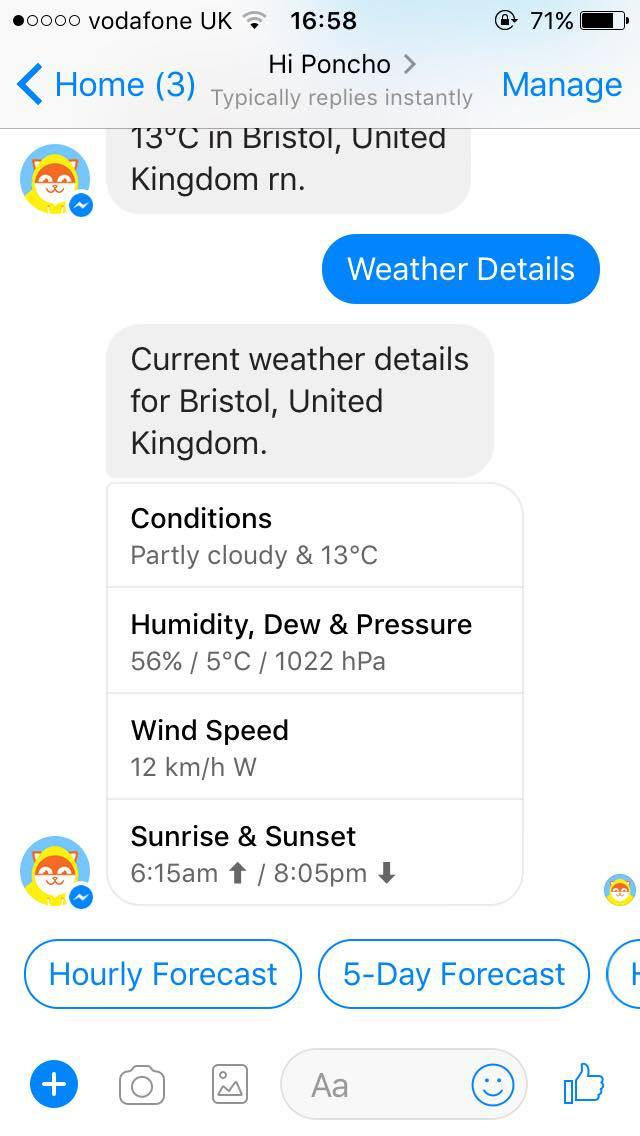
\includegraphics[width=3.2in]{../resources/poncho.jpg}
    \caption{Poncho: A Facebook Messenger Weather Chatbot}
    \label{fig:poncho}
\end{figure}

  \subsection{Design Considerations}
    - Setup:
      - Setup the bot via a messaging platform, such as fb messenger
    - Trigger:
        - Either A, certain configured time of the day
        -        B: No trigger
        -        C: Around a specific time
    - Action:
      - Choose habit from list of habits
      - Perform
      - Use app to track the action
    - Reward:
      - You get one of these rewards, based on modalitiy selected
      - Vision
        - Through message, of an image or gif
        - Could be: App, or message, gif
      - Audatory
        - Through phone via bot, link to mp3/spotify/apple music
        - Could be: App
      - Tactic
        - Through wearable
        - Could be: App, bot triggers wearbale alarm



  \subsection{User Flow}
      - Pre-Start
        - Choose daily habit type from list of X, e.g. 1 press up before breakfast
        - Enable notifications or fitbit if chosen
        - Time action / reward, variable rewards, e.g. then work out average time to send, or none
      - Start:
        - New day
        - @ trigger time, send reminder, if set, notification
        - Open notification, do habit, press tracked
        - Get reward type

% \newpage
% TODO maybe move this into design
%   \subsection{Implementation}
%     - Web app could be chosen because its easiest and achievable, however the ease of use with a chatbot, integrated into fb messenger means everyone can use it on multiple devices. The addition, means that people get used to the UI.
%   \subsubsection{Technology}
%       - 3 Types:
%         1. specific apps
%           - Bad cuz takes a long time
%         2. Web Apps
%           - Still another app
%         3. Chatbot
%           - Good useful
%       - Android/iOS/chatbot specific notifications from web app
%       - Save to home screen
%   \subsubsection{Implementing Rewards}
%       - Vision
%         - Send notification
%         - Show nice visuals
%       - Audio
%         - Send notification
%         - Play uplifting music
%       - Tactic
%         - A.P.I. sets wearable alarm
%         - Wearable (fitbit) issues and tracks alarm times
%     \subsection{Components}
%       [app] -------> (Database) -----> at certain time ---> Send notification to trigger type of reward
%       [ big button that says track]
%       taskname textbox

% \newpage
% \section*{Implementation old}

% Habit formation, Don't Kick the Habit \cite{article_dont_kick_habit}, stopping the behaviour when one stops using behaviour change apps.
% Measuring Habit strength \cite{article_habit_strength} \cite{article_habit_measurement}.

% Multi-Modal interaction, using multiple modalities for habit formation \cite{}, using wearable devices, such as a Fitbit device is plausible for a study \cite{article_wearable_good}.

% Gamification elements \cite{f2p_games_how_to}, can we use any elements from Free-To-Play games?